\documentclass{beamer}
\usetheme{Berlin}
\usepackage[utf8]{inputenc}
\usepackage[russian]{babel}
\usepackage{amsfonts}
\usepackage{natbib}
\usepackage{upquote}
\usepackage{datetime}

\newcommand{\mA}{\mathbf{A}}
\newcommand{\mB}{\mathbf{B}}
\newcommand{\mY}{\mathbf{Y}}
\newcommand{\mU}{\mathbf{U}}
\newcommand{\mV}{\mathbf{V}}
\newcommand{\mE}{\mathbf{E}}
\newcommand{\mQ}{\mathbf{Q}}
\newcommand{\mS}{\mathbf{S}}
\newcommand{\mR}{\mathbf{R}}
\newcommand{\mP}{\mathbf{P}}
\newcommand{\mL}{\mathbf{\Lambda}}
%vectors
\newcommand{\va}{\mathbf{a}}
\newcommand{\vb}{\mathbf{b}}
\newcommand{\vv}{\mathbf{v}}
\newcommand{\vz}{\mathbf{z}}
\newcommand{\ve}{\mathbf{e}}
\newcommand{\tuple}[1]{\langle{#1}\rangle}
\newcommand*\rfrac[2]{{}^{#1}\!/_{#2}}

\beamertemplatenavigationsymbolsempty
\title{LATENT VARIABLES IN STATISTICS AND THEIR APPLICATION TO A PROBLEM OF
RATING ESTIMATION }
\author{A.M. Andronov, A. A.Ressin and K. Pilyushonoka}
\subtitle{Experimental study}

\begin{document}
\setbeamertemplate{footline}[frame number]
\begin{frame}
\titlepage
\end{frame}

\begin{frame}
\frametitle{Data volume}
Total in Netflix Prize\citep{netflix} Dataset: 
\begin{itemize}
  \item movies -- 17,770;
  \item customers -- 480,189;
  \item cross-scores -- 100,480,507. 
\end{itemize}
\end{frame}

\begin{frame}
\frametitle{Data volume analysis}
\begin{itemize}
  \item Histogram of customer awareness of movies   
  	\begin{itemize}
  	\item X -- user awareness: count of different movies watched by a single
  	customer;
  	\item Y -- count of users with given awareness.
	\end{itemize}
  \item Histogram of movies popularities
  	\begin{itemize}
  	\item X -- movie popularity: count of different customers that watched a
  	single movie;
  	\item Y -- count of movies with given popularity.
	\end{itemize}
\end{itemize}
\end{frame}

\begin{frame}
\frametitle{Data volume analysis}
\framesubtitle{Users awareness}
\begin{figure}[h] 
    \includegraphics[width=\linewidth]{users_awareness.png}
\end{figure}
\end{frame}

\begin{frame}
\frametitle{Data volume analysis}
\framesubtitle{Users awareness (log-scale)}
\begin{figure}[h] 
    \includegraphics[width=\linewidth]{users_awareness_logscale.png}
\end{figure}
\end{frame}

\begin{frame}
\frametitle{Data volume analysis}
\framesubtitle{Movies popularity}
\begin{figure}[h] 
    \includegraphics[width=\linewidth]{movies_popularity.png}
\end{figure}
\end{frame}

\begin{frame}
\frametitle{Data volume analysis}
\framesubtitle{Movies popularity (log-scale)}
\begin{figure}[h] 
    \includegraphics[width=\linewidth]{movies_popularity_logscale.png}
\end{figure}
\end{frame}

\begin{frame}
\frametitle{Data volume analysis}
\framesubtitle{Summary}
\begin{itemize}
  \item Awareness:
  	\begin{itemize}
    \item the most frequent (4014 cases) awareness for user is 18;
    \item average -- 209.25;
    \item standard deviation -- 302.33. 
    \end{itemize}
  \item Popularity:
  	\begin{itemize}
    \item the most frequent (64 cases) popularity for movie is 120;
    \item average -- 5654.50; 
    \item standard deviation -- 16909.67. 
    \end{itemize}
  \item Score fill ratio: 1.18\%.
\end{itemize}
\end{frame}

\begin{frame}
\frametitle{Data availability}
\framesubtitle{Sparse matrix visual representation: grayscale}
\begin{columns}[T] % align columns
\begin{column}{.48\textwidth}
\begin{figure}[h] 
    \includegraphics[width=5cm]{usual_grayscale_0.png}
\end{figure}
usual
\end{column}%
\hfill%
\begin{column}{.48\textwidth}
\begin{figure}[h] 
    \includegraphics[width=5cm]{log_grayscale_0.png}
\end{figure}
log-scale
\end{column}%
\end{columns}
\end{frame}

\begin{frame}
\frametitle{Data presence}
\framesubtitle{Sparse matrix visual representation: rainbow}
\begin{columns}[T] % align columns
\begin{column}{.48\textwidth}
\begin{figure}[h] 
    \includegraphics[width=5cm]{usual_0.png}
\end{figure}
usual
\end{column}%
\hfill%
\begin{column}{.48\textwidth}
\begin{figure}[h] 
    \includegraphics[width=5cm]{log_0.png}
\end{figure}
log-scale
\end{column}%
\end{columns}
\end{frame}

\begin{frame}
\frametitle{Solid submatrix of given sparse matrix}
\begin{itemize}
  \item Let $I$ and $J$ are set of customers and objects indices respectively.
The task is to find such $I^* \subseteq I$ and $J^* \subseteq J$, that 
$\forall i \in I^* \forall j \in J^*  \exists  y_{ij}$, where $y_{ij}$ is
score of object $j$ given by user $i$ and $|I^*||J^*| \rightarrow max$.
\item The problem is NP-complete, because it is form of famous Clique Problem.
\item Need for problem relaxation: maximize submatrix density for given
submatrix size $|I^*|\times |J^*|$: 
\begin{equation*}
|I^*||J^*| - |\{y_{ij}: i \in I^*, j \in J^*, \exists y_{ij} \}|
\rightarrow min.
\end{equation*}
\item The problem still is NP-complete, but now it has heuristical solution.
\end{itemize}
\end{frame}

\begin{frame}
\frametitle{Heuristical solution}
\begin{itemize}
  \item Let $\mQ = \{q_{ij}\}_{n \times m}$ -- binary matrix representing data
  availability.
  \item Let introduce $\phi_{i}$ -- authority factors of users, and $\tau_{j}$
  -- authority factors of movies, such that
  \begin{equation*}
\phi_{i}  = \frac{\sum\limits_{j = 1}^m\tau_{j}
  q_{ij}}{\sum\limits_{j=1}^m q_{ij}},
\text{ and }
\tau_{j}  = \frac{\sum\limits_{i = 1}^n\phi_{i} q_{ij}}{\sum\limits_{j=1}^m
q_{ij}}.  
  \end{equation*}
  \item Take $I^*$ as first $\hat{n}$  indices $i$ from $I$ with maximal
  $\phi_i$, and $J^*$ as first $\hat{m}$  indices $j$ from $J$ with maximal
  $\tau_j$, i.e.
  \begin{equation*}
  I^* = \{i_1, \ldots, i_{\hat{n}}\} \text{ where } \phi_{i_1}  > \ldots > \phi_{i_{\hat{n}}} >
 \ldots > \phi_{i_{n}}, 
  \end{equation*}
  \begin{equation*}
  J^* = \{j_1, \ldots, j_{\hat{n}}\} \text{ where } \tau{j_1}  > \ldots >
  \tau{j_{\hat{n}}} > \ldots > \tau{j_{n}}.
  \end{equation*}  
  
\end{itemize}
\end{frame}

\begin{frame}
\frametitle{The idea behind authority factors}
We can treat binary matrix $\mQ$ as adjacency matrix of some bipartite graph
$G$, which vertices are splitted in two disjoined sets $U$ and $V$.
\begin{columns}[T] % align columns
\begin{column}{.48\textwidth}
\begin{figure}[h] 
    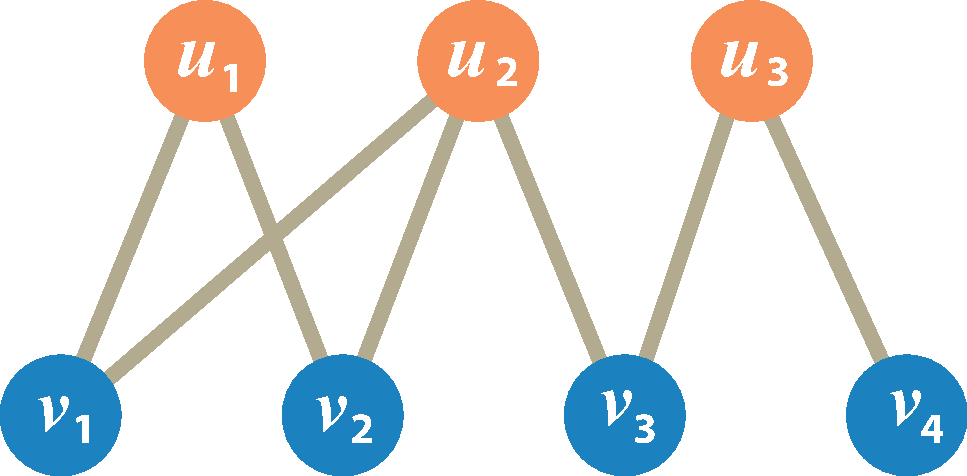
\includegraphics[width=5cm]{DemoGraphQ.pdf}
\end{figure}
\end{column}%
\hfill%
\begin{column}{.48\textwidth}
\begin{eqnarray*}
\mQ = 
\left(
 \begin{array}{cccc}
    1& 1& 0& 0\\
    1& 1& 1& 0\\
    0& 0& 1& 1\\
  \end{array}
   \right)
\end{eqnarray*}
\end{column}%
\end{columns}
Lets consider random walk process on graph $G$, with equal probabilities for
each outgoing arc. 
Thus transition from set $U$ to set $V$ can be represented in form of
stochastic matrix $\mQ_1$ and transition from $V$ to $U$ as $\mQ_2^T$\ldots
\end{frame}

\begin{frame}
\frametitle{The idea behind authority factors}
Thus transition from set $U$ to set $V$ can be represented in form of
stochastic matrix $\mQ_1$ and transition from $V$ to $U$ as $\mQ_2^T$
\begin{columns}[T] % align columns
\begin{column}{.48\textwidth}
\begin{figure}[h] 
    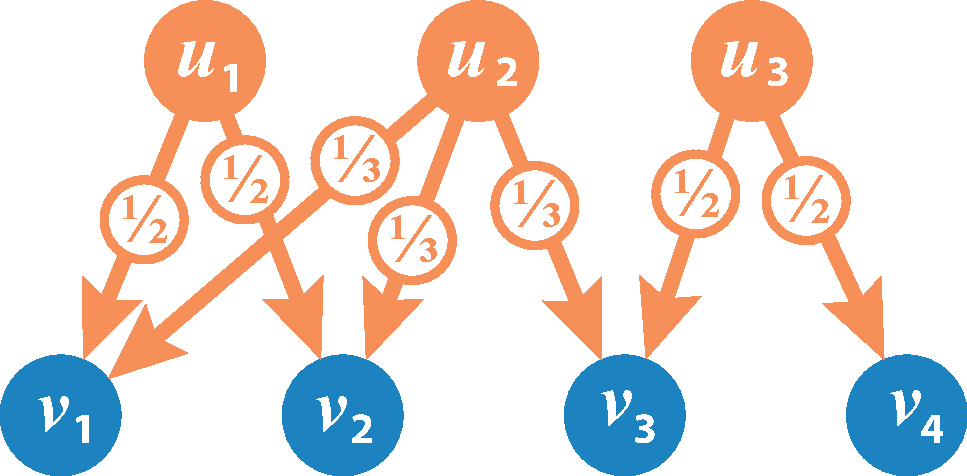
\includegraphics[width=5cm]{DemoGraphQ1.pdf}
\end{figure}
\end{column}%
\hfill%
\begin{column}{.48\textwidth}
\begin{eqnarray*}
\mQ_1 =  \left(
 \begin{array}{cccc}
    \rfrac{1}{2} & \rfrac{1}{2}& 0& 0\\
    \rfrac{1}{3}& \rfrac{1}{3}& \rfrac{1}{3}& 0\\
    0& 0& \rfrac{1}{2}& \rfrac{1}{2}\\
  \end{array}
   \right)
\end{eqnarray*}

\end{column}%
\end{columns}
\end{frame}

\begin{frame}
\frametitle{The idea behind authority factors}
Thus transition from set $U$ to set $V$ can be represented in form of
stochastic matrix $\mQ_1$ and transition from $V$ to $U$ as $\mQ_2^T$
\begin{columns}[T] % align columns
\begin{column}{.48\textwidth}
\begin{figure}[h] 
    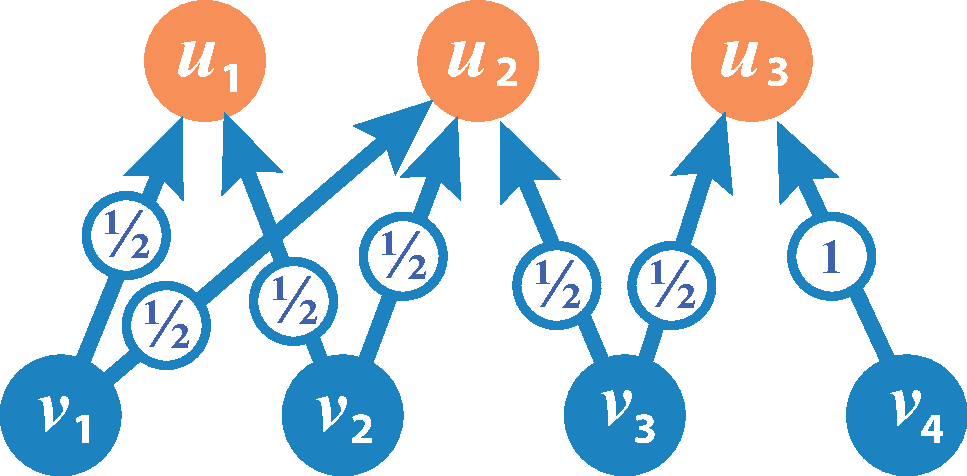
\includegraphics[width=5cm]{DemoGraphQ2.pdf}
\end{figure}
\end{column}%
\hfill%
\begin{column}{.48\textwidth}
\begin{eqnarray*}
\mQ_2^T = \left(
 \begin{array}{ccc}
    \rfrac{1}{2}& \rfrac{1}{2}& 0\\
    \rfrac{1}{2}& \rfrac{1}{2}& 0\\
    0& \rfrac{1}{2}& \rfrac{1}{2}\\
    0& 0& 1\\
  \end{array}
   \right)
\end{eqnarray*}
\end{column}%
\end{columns}


\end{frame}
\begin{frame}
\frametitle{The idea behind authority factors}
\begin{itemize}
  \item In this setting authority factors $\phi_i$ and $\tau_j$ are essentialy
stationary probabilities for random walk process defined by
stohastic matrices $\mQ_1\mQ_2^T$ and $\mQ_1^T\mQ_2$ respectively and can be
described by following equations:
 \begin{eqnarray*}
 \phi = \mQ_1 \tau, \text{ and } \tau = \mQ_2^T \phi.  
 \end{eqnarray*}
  \item The algoritm is very similar to one used by Google which assigns
PageRank authority factor to each web-page in the Internet as logarithm of stationary
probability for random walk through the Internet graph defined by hyperlinks.
\end{itemize}
\end{frame}

\begin{frame}
\frametitle{Data availability}
\framesubtitle{Densities before and after sorting by authority factors}
\begin{columns}[T] % align columns
\begin{column}{.48\textwidth}
\begin{figure}[h] 
    \includegraphics[width=5cm]{usual_grayscale_0.png}
\end{figure}
initial
\end{column}%
\hfill%
\begin{column}{.48\textwidth}
\begin{figure}[h] 
    \includegraphics[width=5cm]{usual_grayscale_5.png}
\end{figure}
after 5 iterations
\end{column}%
\end{columns}
\end{frame}

\begin{frame}
\frametitle{Data availability}
\framesubtitle{Densities before and after sorting by authority factors}
\begin{columns}[T] % align columns
\begin{column}{.48\textwidth}
\begin{figure}[h] 
    \includegraphics[width=5cm]{usual_0.png}
\end{figure}
initial
\end{column}%
\hfill%
\begin{column}{.48\textwidth}
\begin{figure}[h] 
    \includegraphics[width=5cm]{usual_5.png}
\end{figure}
after 5 iterations
\end{column}%
\end{columns}
\end{frame}

\begin{frame}
\frametitle{Data availability}
\framesubtitle{Densities before and after sorting by authority factors:
log-scale}
\begin{columns}[T] % align columns
\begin{column}{.48\textwidth}
\begin{figure}[h] 
    \includegraphics[width=5cm]{log_grayscale_0.png}
\end{figure}
initial
\end{column}%
\hfill%
\begin{column}{.48\textwidth}
\begin{figure}[h] 
    \includegraphics[width=5cm]{log_grayscale_5.png}
\end{figure}
after 5 iterations
\end{column}%
\end{columns}
\end{frame}

\begin{frame}
\frametitle{Data availability}
\framesubtitle{Densities before and after sorting by authority factors:
log-scale}
\begin{columns}[T] % align columns
\begin{column}{.48\textwidth}
\begin{figure}[h] 
    \includegraphics[width=5cm]{log_0.png}
\end{figure}
initial
\end{column}%
\hfill%
\begin{column}{.48\textwidth}
\begin{figure}[h] 
    \includegraphics[width=5cm]{log_5.png}
\end{figure}
after 5 iterations
\end{column}%
\end{columns}
\end{frame}

\begin{frame}
\frametitle{Submatrix selection}
\framesubtitle{}
\begin{itemize}
  \item $500 \times 500$ -- upper left corner of data sorted according to
  authority factors;
  \item missing ratio -- 7\% (score fill ratio increased from 1.18\% to 93\%).
\end{itemize}
\begin{columns}[T] % align columns
\begin{column}{.48\textwidth}
\begin{figure}[h] 
    \includegraphics[width=3.5cm]{scores_500x500.png}
\end{figure}
scores
\end{column}%
\hfill%
\begin{column}{.48\textwidth}
\begin{figure}[h] 
    \includegraphics[width=3.5cm]{missing_500x500.png}
\end{figure}
missing data (black pixels)
\end{column}%
\end{columns}
\end{frame}

\begin{frame}
\frametitle{Interpolating missing data}
\begin{itemize}
  \item Interpolation aim:
  \begin{itemize}
    \item provide solid matrix for singular value decomposition for checking
    hypothesis about low rank approximation;
    \item not to predict missing data(!). 
    \end{itemize}
    \item Lets denote $I(j) = \{i: \exists y_{ij}\}$ and $J(i) = \{j: \exists
    y_{ij}\}$.
    \item Interpolation algorithm:
    \begin{equation*}
    \tilde{y_{ij}} = \frac{\sum\limits_{k \in I(j)} y_{kj} + \sum\limits_{k \in J(i)}
    y_{ik}}{|I(j)| + |J(i)|}. 
    \end{equation*}
    \item Patch matrix $\hat{\mY} = \{\hat{y_{ij}} \}$ where
    \begin{equation*}
    \hat{y_{ij}} = 
    \begin{cases} 
     y_{ij} \text{-- if } y_{ij} \text{is available};\\
    \tilde{y_{ij}} \text{ -- otherwise};
    \end{cases}
    \end{equation*} 
\end{itemize}
\end{frame}

\begin{frame}
\frametitle{Singular Values of matrix $\hat{\mY}$}
\begin{columns}[T] % align columns
\begin{column}{.48\textwidth}
\begin{figure}[h] 
    \includegraphics[width=5cm]{svd.png}
\end{figure}
all values
\end{column}%
\hfill%
\begin{column}{.48\textwidth}
\begin{figure}[h] 
    \includegraphics[width=5cm]{svd_10.png}
\end{figure}
first 10 values
\end{column}%
\end{columns}
\end{frame}

\begin{frame}
\frametitle{Singular Values of matrix $\hat{\mY}$: logscale}
\begin{columns}[T] % align columns
\begin{column}{.48\textwidth}
\begin{figure}[h] 
    \includegraphics[width=5cm]{svd_log.png}
\end{figure}
all values
\end{column}%
\hfill%
\begin{column}{.48\textwidth}
\begin{figure}[h] 
    \includegraphics[width=5cm]{svd_log_10.png}
\end{figure}
first 10 values
\end{column}%
\end{columns}
\end{frame}

\begin{frame}
\frametitle{Dependency $|\hat{\mY} - \tilde{\mY}|_F$ over approximation rank
$k$}

\begin{columns}[T] % align columns
\begin{column}{.48\textwidth}
\begin{figure}[h] 
    \includegraphics[width=5cm]{svd.png}
\end{figure}
all values
\end{column}%
\hfill%
\begin{column}{.48\textwidth}
\begin{figure}[h] 
    \includegraphics[width=5cm]{svd_10.png}
\end{figure}
first 10 values
\end{column}%
\end{columns}
\end{frame}


\begin{frame}[allowframebreaks]
\bibliographystyle{ieeetr}
\bibliography{references}
\end{frame}

\begin{frame}
\frametitle{}
\framesubtitle{}
\begin{itemize}
  \item 
\end{itemize}
\end{frame}

\end{document}
